\section{Knowledge Association Network}
\label{kan}
It has long been thought that when humans measure the relatedness between a pair of words,
a deeper reasoning which requires a large amount of knowledge is triggered to compare the concepts behind the words.
There are many data resources that contain concepts which are associate with words such as Wikipedia, Wordnet and DBPedia etc.
Wordnet provides precise lexical information but lacks adequate semantic information.
Wikipedia is a large corpus where a page describes a concept.
DBPedia contains abundant structured knowledge consisting of a great number of facts which are extracted from wikipedia. 

Inspired by the free association network in semantic relatedness between two words\cite{aaai/GongXH18,aaai/ZhangZH15}, 
we consider the DBPedia as concepts database to avoid the significant preprocessing and data transformation efforts in wikipedia. 
To measure the relatedness between two entities, we consider two major factors in DBPedia: attributes information and topological structure. 
The attributes of an entity include the properties, categories, ontology information and some other information which enhances
the entity itself. Topological structure reflects the relations between other
entities on the basis of a special predicate in DBPedia: \emph{WikiPageRedirectOf}.
That means if two entities are connected by this predicate, they appear in the same Wikipedia page.

\begin{figure}
    \flushleft
    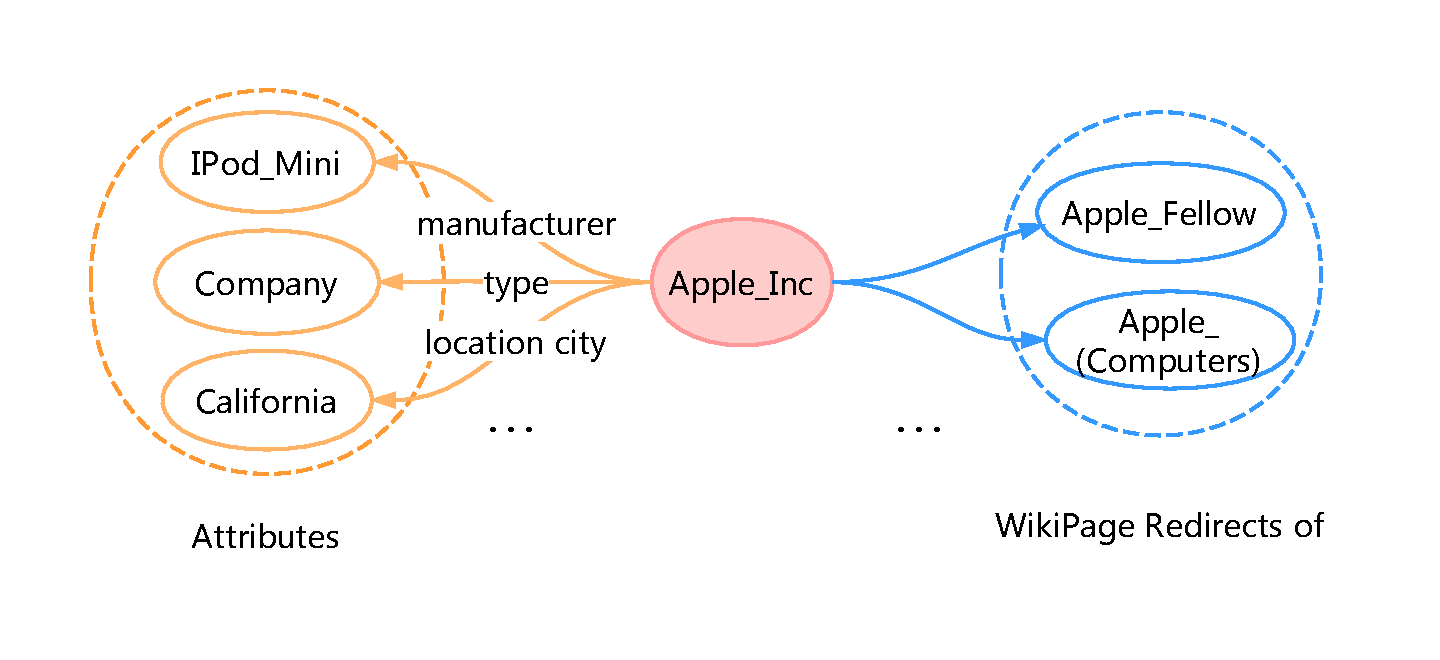
\includegraphics[width=0.5\textwidth]{pic/kg.pdf}\\
    \caption{The semantics around an entity}
    \label{kg}
\end{figure}

There is an example in figure \ref{kg}, for the technology company Apple which is described
as \emph{Apple Inc} in DBPedia, we get its attributes, that is, "Apple is the manufacturer of IPod Mini(properties)"; "Apple is a company(categories)" and etc.
And the relationship descriptions(\emph{predicates in triples)} are named on the basis of ontology language that contains affluent semantics.
In the aspect of links among other co-occurrence entities, there are entities \emph{Apple\_Fellow} and \emph{Apple\_(Company)} in accordance with the
special relationship \emph{WikipageRedirectOf}.

DBPedia contains natural attributes network structure and abundant semantics.
We define a set of entities $\mathit{E_w=\{e_1, e_2, ..., e_i\}}$ that represent the semantics behind a word and $e_i$ is an entity in DBPedia.
We refer to the attributes of an entity as an attributes graph $\mathit{G_{attr}=\{a_1, a_2, ..., a_j\}}$ and define topological structure as 
$\mathit{G_{t}=G(E, R_{redirect})}$, where $a_i$ denotes an attribute and $E$ is a set of entities, $R_{redirect}$ is the edge set formed by
\emph{WikiPageRedirectOf}.

\subsubsection{Definition}
\emph{Knowledge association network can be modelled as a graph $G=(W, E, R)$ where $w$ is the word set in vocabulary, $E$ is the entity set contained in DBPedia,
and edge set $R$ denotes the relationships including word-to-word($R_{w}$), entity-to-entity($R_{e}$), and word-to-entity($R_{we}$).}

\subsubsection{Network Construction}
A necessary work in network construction is to build the mapping between words and concepts(entities). 
This comes in handy in Wikipedia pages. The mapping between words and Wikipedia page reflects 
the structure of association network naturally, and fortunately there is a 1-to-1 match between entity in DBPedia and page in Wikipedia.
In other words, Wikipedia page and it's corresponding DBPedia entity elaborate the same concept.
Consequently we can construct knowledge association network based on this natural mapping.

There is a special attribute called \emph{WikipageID} that reflects the mapping between entities in DBPedia and pages
in Wikipedia by the unique id.
The id can be obtained by the \emph{Gensim}\footnote{https://radimrehurek.com/gensim/wiki.html} that is a free Python
library designed to automatically extract semantic topics from documents. By the aid of unique page id,
we get the unique corresponding entity in DBPedia by SPARQL endpoint\footnote{http://dbpedia.org/sparql}.
For example, the id of Wikipedia page \emph{Apple Inc} is $856$, we can use a simple query to get the unique entity name \emph{Apple\_Inc}:

\begin{lstlisting}[basicstyle=\fontsize{9}{11}\ttfamily]
PREFIX dbo: <http://dbpedia.org/ontology/>
SELECT ?E WHERE {
    ?E dbo:wikiPageID 856.
}
\end{lstlisting}

